\documentclass[opre,dblanonrev]{informs4}
\usepackage{amsmath,amssymb,graphicx,booktabs,natbib,url}
\OneAndAHalfSpacedXII
\EquationsNumberedThrough
\TheoremsNumberedThrough
\graphicspath{{../experiments/reconstruction_v3/}}
\providecommand{\newblock}{\ }
\MANUSCRIPTNO{}
\makeatletter
\def\theARTICLETOP{}
\def\theARTICLEABSTRACT{%
  \vspace*{10pt}%
  \begin{minipage}[t]{\textwidth}\ABSfont
    \noindent\theABSTRACT\endgraf
    \vskip5pt
    \theKEYWORDS
  \end{minipage}\par\vspace*{12pt}}
\makeatother

\begin{document}
\RUNAUTHOR{Anonymous}
\RUNTITLE{Causal Diagnostics for Transit Routing}
\TITLE{Causal Diagnostics for Candidate Selection in Stochastic Transit Routing}
\ARTICLEAUTHORS{\AUTHOR{Anonymous}\AFF{Affiliation withheld for review}}
\ABSTRACT{%
A missed vehicle can reflect an omitted feasible connection, a poor choice
among admitted connections, or a continuation forecast that assigns the wrong
value to recovery. We distinguish these mechanisms using a committed boarding
model with fixed vehicle outcomes, time-stamped local observations, and a
common capped journey loss. Two exact multileg examples on Z\"urich timetable
fragments isolate a loss from omitting a same-vehicle continuation and a loss
from decision-making within a candidate set. A 35-date, 18-OD generated panel
calibrated to route-identified forecasts gives mean losses of 27.05 minutes for
a feasible nominal policy and 25.88 for a history-conditioned rollout. Their
mean compute times are 3.59 and 16.24 seconds. A separate deadline stress panel
slightly favors the nominal policy. Matched transition budgets on six further
conditions show where smaller candidate menus can save time. A two-date
measured railway replay and a held-out endpoint check delimit the realism of
the generated vehicle model. The results support evaluating candidate
admission and continuation scoring separately before committing to a candidate
compression algorithm.}
\KEYWORDS{stochastic transit routing, partial information, recourse, evaluation}
\maketitle

\section{Decision problem and related work}

A traveler has arrived at a stop, possibly on a vehicle that continues toward
the destination. They may stay with that vehicle, change to a different one, or
wait for information. The traveler's choice changes which events can be
observed before the next commitment. A ranking that removes a boardable
same-vehicle segment before scoring can therefore fail even when its
conditional failure probabilities are accurate. Conversely, a candidate menu
can contain both viable alternatives while their relative costs depend on the
value of waiting or the action available after a missed departure.

Partial stop-level information and adaptive public transit policies have
established precedents \citep{chenNie,rambha}. \citet{geissmann} give efficient
adaptive policies for independently failing temporal connections, including a
Z\"urich study. \citet{durner} studies realtime delay predictions, stochastic
arrival labels, and several transfer strategies. These results motivate using
a native strict strategy as a comparison and distinguishing its conditional
arrival criterion from a capped journey loss. In a different setting,
\citet{hanasusanto} study a restricted inventory of adaptive plans, while
\citet{silver} use simulation to search over action--observation histories.
Here we use that style of search as a reference, with an explicit transition
budget. Our contribution is the diagnostic comparison on a common execution
contract, including where candidate restriction, scoring and model fidelity
change the interpretation of the results.

\section{Execution contract and continuation values}
\label{sec:contract}

Let $t_0$ be the departure clock and $C$ the deadline in minutes from $t_0$.
The loss is the elapsed time at destination if reached by $t_0+C$, and $C$
otherwise. Each generated world fixes one cancellation and one integer delay
for each trip. The delay shifts the scheduled departure and arrival of each
segment of that trip. Different trips are independent in the fitted city-panel
model. The exact diagnostic fragments can instead couple outcomes by a
persistent regime.

A public history $h$ contains the stop, clock, last arrival, current trip, and
observed vehicle events and attempt feedback. Each local decision publishes up
to five unseen events that have occurred at the stop in the last ten minutes.
A departure at the current minute remains boardable. A different vehicle
requires the minimum transfer time from the previous arrival. Staying on the
same trip incurs no transfer time. A boarding choice commits to at most 12
minutes of waiting after the traveler is ready, subject to the overall
deadline. A one-minute wait defers the commitment. The scheduled departure
lookahead is 25 minutes. Boarding, cancellation, a missed departure and an
expired commitment generate different feedback. A missed attempt reveals that
the vehicle departed too early. The exact departure becomes available only if
it was independently reported. The execution clock uses physical travel and
waiting times. We measure planner wall time separately.

For a first boarding action $c$, write $B$ for boarding within the commitment
window, $p=\Pr(B\mid h,c)$, $A$ for the conditional expected capped loss given
$B$, and $F$ for the corresponding cost after a failed first attempt. The
costs use the same causal continuation policy and include elapsed time from
the common origin. Then
\begin{equation}
 Q(h,c)=pA+(1-p)F . \label{eq:first-boarding}
\end{equation}
A known trip outcome conditions all of its segments. An unknown trip uses a
discrete plug-in delay model conditioned on receipts, missing publications and
attempt feedback. Route fits use online mean and cancellation updates and a
historical delay spread. We integrate $p$ directly on the departure support,
and integrate $A$ directly when the action reaches the destination. A shared
bank of eight worlds estimates the other conditional costs. When a needed
positive-mass branch is missing, one additional draw from that branch changes
only the selected trip, retaining every base world. This exploits the
conditional independence of the fitted trips.

The nominal policy uses conditional mean event times and a feasible timetable
search with waiting. The rollout uses the same nominal policy as its tail,
with the route parameters and candidate menu frozen for that query. Subsequent
simulation decisions update their public trip information. The deployed
policy can also refresh its route parameters and menu. The online shortlist
prioritizes feasible same-trip continuations and admits up to five boardings
and the wait action. An ablation replaces $F$ by $C$ for the current attempt.
Every other transition and tail rule is shared in that comparison.

\section{Candidate and information references}

Let $H$ specify an allowed action set at every future public history. With
the same loss and information, a policy $\pi$ restricted by $H$ satisfies
\begin{equation}
 J(\pi)-J^*_{\rm full}=(J^*_H-J^*_{\rm full})+(J(\pi)-J^*_H).
 \label{eq:gap}
\end{equation}
The first term measures the cost of candidate restriction. The second is the
cost of decisions within the rule. Exact finite-bank dynamic programming
groups worlds by public outcome before selecting a continuation, and uses
the same physical publication rule with either action menu. Knowing a regime
changes the initial mixture while leaving several possible futures. Full
hindsight discloses the world. With a fixed menu, increasing information can
only weakly lower the optimum. This gives separate reference values for
candidate restriction and information availability.

Two four-connection Z\"urich fragments illustrate the distinction. Removing
the through service's same-trip continuation increases the same-information
optimum from 3.625 to 5.75 minutes. A restricted heuristic adds 1.25 minutes.
In a second fragment, deleting a transfer backup leaves the same-information
optimum at 6 minutes, and the restricted heuristic costs 8. Knowing the
current regime gives full and restricted costs of 5.6 and 5.8 minutes.
Hindsight gives 5 minutes for both. The second example uses two possible
future worlds within each known regime. Increasing its horizon from 12 to 30
minutes grows the full reference from 572 to 18,869 information nodes. This
measures exact enumeration on a fragment with a specified world bank.

\section{Forecast-calibrated generated comparisons}

Exact trip identifiers link 189 trips and 2,000 connections to 33 route IDs.
Sampling the archived realtime feeds and deduplicating event revisions
produces 1,027,848 delay forecasts and 109,335 observed trip statuses over 35
dates. Of those statuses, 237 declare cancellation. Daily world parameters
use the target date's delay forecasts and declared service statuses. The
policies use priors built from strictly earlier dates, with a documented
fallback for missing route support. The timetable template deliberately holds
topology fixed across conditions. Its constituent trips span different GTFS
service calendars, which activate 74--176 of its connections per date in the
archived static feed. The 35-date panel therefore describes generated trips
on a common timetable template. Calendar-consistent measured evidence is
reported separately below.

The main experiment evaluates the original 18 OD pairs for each date under
one common generated world, using a 120-minute cap. The four strategies are
an online marginal-label score, native Durner strict, the feasible nominal
policy and the continuation rollout. All face the same exogenous vehicle
outcomes and publication mechanism. Native strict keeps its own objective
and is evaluated under the common capped loss. Table~\ref{tab:chronological}
summarizes 2,520 journeys. The rollout improves on nominal by 1.17 minutes on
average, with 59 improvements, 15 regressions and 556 ties among the 630 OD
conditions. Resampling the 35 generated date groups gives a descriptive
rollout-minus-nominal interval of $[-2.49,-0.30]$ minutes. These generated
groups are distinct from a sample of measured disruptions.

\begin{table}[ht]
\TABLE{Generated 35-date, 18-OD panel\label{tab:chronological}}{%
\begin{tabular}{lrrr}
\toprule
Strategy & Mean loss (min) & Arrival (\%) & Mean compute (s)\\
\midrule
Marginal score & 52.00 & 70.95 & 4.56\\
Durner strict & 61.56 & 63.81 & 4.44\\
Feasible nominal & 27.05 & 95.08 & 3.59\\
Continuation rollout & 25.88 & 95.87 & 16.24\\
\bottomrule
\end{tabular}}{Timing includes initial preparation and all online decisions.
Each date is one generated vehicle world shared across the 18 OD pairs.}
\end{table}

On 12 separate stress conditions, the date-specific delay location is
increased by eight minutes, the standard deviation has a four-minute floor,
and the cancellation probability has a 20\% floor. Across the 60-, 90- and
120-minute caps, nominal and rollout each arrive on 11 conditions and rollout
costs 0.67 minutes more on average at each cap. In another eight generated
conditions with new OD pairs and dates from the earlier forecast model,
nominal costs 31.00 minutes and rollout costs 31.63. Figure~\ref{fig:dates}
shows date variation and the deadline sensitivity. The comparison supports
keeping nominal as a substantive, low-compute reference.

\begin{figure}[ht]
\FIGURE{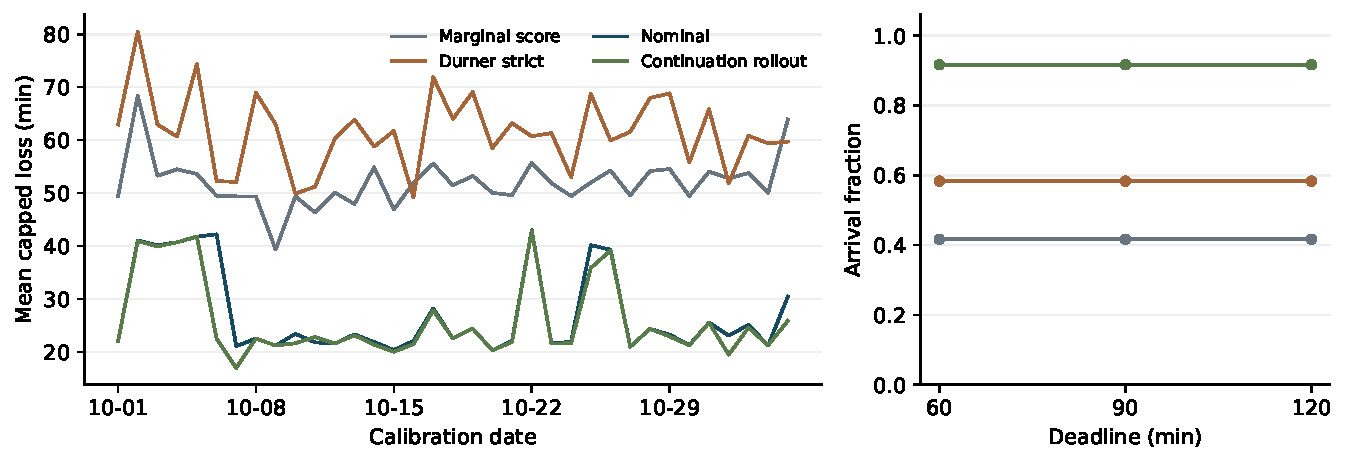
\includegraphics[width=.96\textwidth]{chronological_panel.pdf}}
{Date-level loss and arrival under deadline stress\label{fig:dates}}
{The left panel averages 18 OD pairs per generated world. The right panel
uses 12 shared stress conditions per cap.}
\end{figure}

\section{Matched computation and measured replay}

On six route-identified conditions from three dates we compare unrestricted
physical actions, a frozen initial menu, a smaller frozen menu, and a generic
public-history UCT search. The smaller menu retains five initial labels per
stop and closes the set under trip membership. It retains 1,149--1,508 of
2,000 connections. All planners respect a common upper limit of 128 or 512
committed-model transitions per decision. A rollout estimate uses only
complete common-world rounds over the root actions and falls back to nominal
when none completes. UCT allocates its transition budget over public histories.
At budget 128 the full and smaller-menu mean losses are 31.33 and 31.50
minutes. At 512 they agree on all six journeys with mean 28.67. Mean
end-to-end compute falls from 25.68 to 18.99 seconds at that larger budget.
The matched limit counts transitions. Wall time also includes model setup,
candidate preparation and search overhead. In these six conditions UCT has
the lowest loss at 128 and is worse than full rollout at 512. This comparison
measures a local empirical tradeoff for a bounded approximate search.

\begin{figure}[ht]
\FIGURE{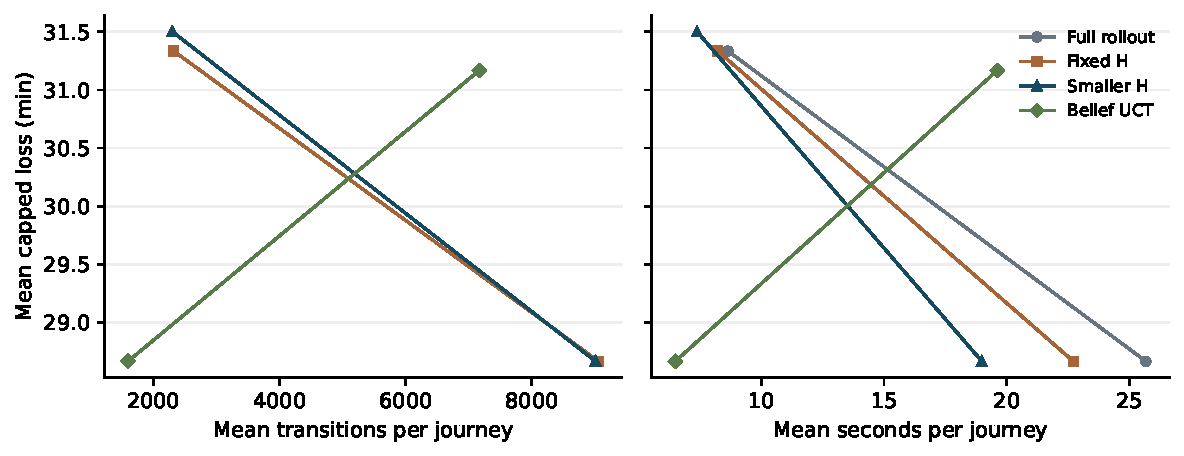
\includegraphics[width=.91\textwidth]{route_id_budget.pdf}}
{Quality and computation at two transition budgets\label{fig:budget}}
{Six paired generated conditions on the route-identified graph. The panels
report actual simulated work and elapsed compute, respectively.}
\end{figure}

Official Swiss actual data \citep{swissactual} provide unambiguous \texttt{REAL} timestamps for
54 SBB endpoints on October 12 and 25. On these endpoints, empirical 90\%
forecast intervals from earlier dates cover 19/30 and 8/24. Observed arrivals
or departures beyond the upper interval endpoint explain most misses. All
27 measured complete legs have different departure and arrival delays, with
a maximum difference of 239 seconds. That directly limits the common-shift
assumption used in the generated comparison.

In a measured two-itinerary replay the traveler reaches Z\"urich HB on S11,
then either stays aboard or transfers to S20 for Z\"urich Hardbr\"ucke. Both
connections are feasible with the specified transfer time on both dates.
Staying on S11 reaches the destination 302 and 233 seconds earlier,
respectively. We separately record the actual times and the forecast
available before each decision. The two measured itineraries identify
realized costs on those services. Citywide evaluation requires measured
competing services and date-specific network coverage.

\section{Implications}

The exact examples show that loss from candidate admission and loss within a
menu can vary independently. The generated city experiments show that a
feasible nominal policy captures much of the improvement over the marginal
score. Explicit rollout adds a smaller and computationally more costly
increment on the main panel, and reverses direction on the stress and fresh
screens. The budgeted experiments show a promising but limited cost reduction
from a smaller menu. A city-scale bound on candidate loss and a cheap stopping
certificate remain separate research questions. The measured endpoints call
for an observation and delay model that allows within-trip variation before
interpreting a generated-policy ranking as a deployment outcome.

\begin{APPENDICES}
\ECHead{Electronic Companion}
\section{First-event scoring and the policy gap}

Equation~\eqref{eq:first-boarding} is the law of total expectation. For fixed
continuation and nonempty branches, subtracting a fitted score gives the exact
decomposition
\begin{equation}
 \widehat Q-Q=(\widehat p-p)(A-F)+\widehat p(\widehat A-A)
                  +(1-\widehat p)(\widehat F-F).
\end{equation}
The conditionally sampled means estimate the fixed fitted tail, and the
choice made by minimizing estimates can still have selection error. If a
branch has zero mass its conditional cost is undefined and its contribution
to the mixture is zero. No estimated probability alone identifies the effect
of choosing a different future tail.

For the within-menu gap in \eqref{eq:gap}, write the one-step optimal
continuation under $H$ as $Q^*_H(h,a)=\mathbb E[c+V^*_H(h')\mid h,a]$, with the
same terminal cost for every policy. The sum of
$Q^*_H(h,a)-V^*_H(h)$ along the executed policy telescopes in expectation to
$J(\pi)-J^*_H$. Thus, if a greedy score has a uniform action error of at most
$\delta(h)$ at each visited history, the per-step advantage is at most
$2\delta(h)$. This is a conditional bound. The sampled fitted score supplies
neither a uniform $\delta(h)$ nor a city-scale exact optimum.

\section{Statistical and formalization scope}

With a Normal--Gamma posterior using rate $\beta_n$, the marginal Student-$t$
scale squared of the mean is $\beta_n/(\alpha_n\kappa_n)$, and its variance for
$\alpha_n>1$ is $\beta_n/[(\alpha_n-1)\kappa_n]$. These differ from the
predictive variance for a future delay. A fixed Lipschitz penalty gives a
Wasserstein upper bound under the usual moment assumptions. An affine
equality additionally requires a feasible translation in the support. This
is standard structure \citep{esfahaniKuhn}. A separate Bayesian risk
formulation requires an explicit parameter-risk functional \citep{linRenZhou}.
For a fixed ambiguity set, the worst-expectation map is nonexpansive in the
supremum norm and discounting gives the discount factor as a contraction
modulus. An undiscounted stochastic shortest path needs its own termination
conditions. The finite reference here uses a finite horizon.

The archived Lean artifact checks abstract statements under their encoded
hypotheses. In particular, its Lipschitz-penalized expectation is defined as
that expression, and the posterior theorem uses a supplied scale or error
condition. A source map in the artifact README records the Lean objects and
their assumptions. Lean 4.28.0 checks all imported proof modules and the main
module with \texttt{lake build +Main:olean}. The checked scope is the abstract
statements. Simulator contracts, forecast calibration, runtime and the
reported comparisons are supported by the executable tests and experiment
receipts.
\end{APPENDICES}

\begin{thebibliography}{9}
\bibitem[Chen and Nie(2015)]{chenNie}
Chen P, Nie YM (2015) Optimal transit routing with partial online information.
\emph{Transportation Research Part B}.
\url{https://doi.org/10.1016/j.trb.2014.11.007}.
\bibitem[Durner(2024)]{durner}
Durner R (2024) \emph{Stochastic Strategies for Public Transport Journeys Based
on Realtime Delay Predictions}. Master's thesis, University of Stuttgart.
\url{https://doi.org/10.18419/opus-14802}.
\bibitem[Geissmann and Gianinazzi(2019)]{geissmann}
Geissmann B, Gianinazzi L (2019) Routing in stochastic public transit networks.
\emph{ATMOS}, article 4. \url{https://doi.org/10.4230/OASIcs.ATMOS.2019.4}.
\bibitem[Hanasusanto et al.(2015)]{hanasusanto}
Hanasusanto GA, Kuhn D, Wiesemann W (2015) K-adaptability in two-stage robust
binary programming. \emph{Operations Research}.
\url{https://doi.org/10.1287/opre.2015.1392}.
\bibitem[Lin et al.(2022)]{linRenZhou}
Lin Y, Ren Y, Zhou E (2022) Bayesian risk Markov decision processes.
\emph{Advances in Neural Information Processing Systems}.
\bibitem[Mohajerin Esfahani and Kuhn(2018)]{esfahaniKuhn}
Mohajerin Esfahani P, Kuhn D (2018) Data-driven distributionally robust
optimization using the Wasserstein metric. \emph{Mathematical Programming}
171:115--166.
\bibitem[Rambha et al.(2016)]{rambha}
Rambha T, Boyles SD, Waller ST (2016) Adaptive transit routing in stochastic
time-dependent networks. \emph{Transportation Science}.
\url{https://doi.org/10.1287/trsc.2015.0613}.
\bibitem[Silver and Veness(2010)]{silver}
Silver D, Veness J (2010) Monte-Carlo planning in large POMDPs.
\emph{Advances in Neural Information Processing Systems}.
\bibitem[Open Data Platform Mobility Switzerland(2023)]{swissactual}
Open Data Platform Mobility Switzerland (2023) Actual data, October 2023
archive. \url{https://archive.opentransportdata.swiss/istdaten/2023/ist-daten-2023-10.zip}.
\end{thebibliography}

\end{document}
